% GENERAL INFORMATION: HardwareX is an open access journal established to promote free and open source designing, building and customizing of scientific infrastructure (hardware). For more details on best practices for sharing open hardware see http://www.oshwa.org/sharing-best-practices/

\documentclass[11pt, letterpaper]{article}
\usepackage[utf8]{inputenc}
\usepackage{amsmath}
\usepackage[margin=1.5cm]{geometry}
\usepackage{titlesec}
\usepackage{tabu}
\usepackage{enumitem}
\usepackage{amssymb}
\usepackage{xcolor}
\usepackage{graphicx}
\newlist{selectlist}{itemize}{2}
\setlist[selectlist]{label=$\square$,leftmargin=*,noitemsep,topsep=0pt}


\usepackage{listings}
\lstset{
    language=C++, % Or C, depending on your preference for highlighting
    basicstyle=\small\ttfamily,
    numbers=left,
    numberstyle=\tiny\color{gray},
    showspaces=false,
    showtabs=false,
    breaklines=true,
    breakatwhitespace=true,
    tabsize=4,
    captionpos=b,
    frame=single,
    frameround=tttt,
    framesep=5pt,
    rulesepcolor=\color{gray},
    backgroundcolor=\color{white},
    commentstyle=\color{green!50!black},
    keywordstyle=\color{blue},
    stringstyle=\color{red!50!black},
    identifierstyle=\color{black},
}

\usepackage{lmodern}

\usepackage[backend=biber]{biblatex}
\addbibresource{references.bib}

% \bibliographystyle{plain}
% \renewcommand\bibname{\itareferencesnamebabel} %renomear título do capítulo referências
% \bibliography{references}

\usepackage{hyperref}
\hypersetup{
    colorlinks=true,
    linkcolor=blue,
    filecolor=magenta,      
    urlcolor=blue,
    citecolor=teal,
}
 
\urlstyle{same}

\newcommand{\red}[1]{{\color{red}#1}}

% Set up the section label formatting
\titleformat{\section}[block]{\hspace{1em}\bfseries}{\thesection.}{0.5em}{} 
\titleformat{\subsection}[block]{\hspace{1em}}{\thesubsection}{0.5em}{}

\begin{document}
% Create the title block
\begin{flushleft}

  {\Huge \bf A flying capacitor three-cell voltage converter for studies in the control of switched systems}

  \setlength{\parindent}{0pt}
  \setlength{\parskip}{10pt}
  % \textbf{\large HardwareX article template}

  %Insert title
  %Max. 20 words. A good title should contain the fewest possible words that adequately describe the content of a paper.

  %Insert Authors
  \textbf{Daniel Vieira, Roberto Kawakami Harrop Galvão*, José Roberto Colombo Júnior}

  % \textit{List all authors. Please mark the corresponding author with (*)

  %Insert Affiliations
  \textbf{Instituto Tecnológico de Aeronáutica, Electronics Engineering Division, 12228-900, São José dos Campos, SP - Brazil}

  %  \textit{Please include the full address of each author institution}

  %Insert Contact Email
  %Include institutional email address of the corresponding author
  \textbf{kawakami@ita.br}



  % \textit{Institutional email address preferred. If you have a Twitter handle, please add it here ‘twitter: \@....’}

  %Insert Abstract
  %Max. 200 words. Remember that the abstract is what readers see first in electronic abstracting and indexing services. This is the advertisement of your article. Make it interesting, and easy to be understood. Be accurate and specific, keep it as brief as possible.
  \textbf{Abstract}\\ \textit{
    The challenges associated with implementing controllers for switched systems often arise from the high cost and complexity of the required hardware.
    This paper addresses that barrier by presenting a low-cost circuit for a three-cell voltage converter specifically designed for the experimental
    study of switched-mode control. The proposed solution uses standard, easily accessible electronic components, making it an ideal platform for
    educational and research purposes. At the heart of the control architecture is an ESP32 microcontroller, which provides the necessary real-time
    capabilities to generate precise signals for the switched actuators. This approach aims to provide a practical and easy-to-implement solution for
    developing and testing control algorithms, thus lowering the entry barrier for students and researchers in the field.
    This work contributes a valuable tool that bridges the gap between the theoretical aspects of switched systems and their accessible,
    hands-on application.}

  %Insert Keywords
  % At least 3 keywords. There is no limit on the no. of keywords you can list. Please remember that effective keywords should not repeat words appearing in your title, and should be neither too general nor too narrow.
  \textbf{Keywords}\\ \textit{Voltage Converter; Low-Cost Circuit; ESP32 Microcontroller; Switched-mode control;}

  \red{To do list:
    \begin{itemize}
      \item Fotos e biografias.
      \item Terminar contextualização na seção 1.
      \item Hardware description: Explicar o porquê dos dois mosfets para implementar as chaves do meio.
      \item Escolher o repositório.
      \item Preencher a tabela de design files.
      \item Preencher a build instructions sucintamente. Falar do uso do KiCad para exportar os arquivos de PCB (comentar o caminho para gerar o arquivo necessário para o fabricante da PCB). Explicar que há vias que podem ser usadas para soldar os componentes THT por baixo, se os furos não estiverem metalizados. Comentar que os componentes THT passivos podem ser soldados por cima ou por baixo. Comentar sobre o uso de soquete para a ESP. Comentar sobre o uso de soquetes para os CIs e os mosfets. Comentar sobre o uso de tuxinhos se forem usados soquetes para os mosfets. Comentar sobre o uso de jumper wires para os pontos de teste. Comentar a instalação dos rubber pads. Tirar nova fotografia.
      \item Operation instructions: Explicar o uso do software com telas passo-a-passo. Mencionar o uso dos pontos de teste para medida com osciloscópio.
      \item Seção 8: \red{Mencionar valores de tempo usados no código do exemplo.}
      \item Colocar subsection de Conclusion na seção de Validation and characterization.
      \item Tela do osciloscópio:  Apresentar vc1, v2, vr durante a transição entre dois valores diferentes de alpha. Apresentar a tela do osciloscópio associada.
      \item Tela do software.
    \end{itemize}
  }


  \newpage
  \textbf{Specifications table}\\
  \textit{Please replace the italicizied instructions in the right column of the table with the relevant information about your hardware.}
  \vskip 0.2cm
  \tabulinesep=1ex
  \begin{tabu} to \linewidth {|X|X[3,l]|}
    \hline  \textbf{Hardware name}                                        & \textit{ESP32 C++ controlled three-cell converter}
    %Please specify the name of the hardware that you invented / customized
    \\
    \hline \textbf{Subject area}                                          &                                                    %
    % Please state the subject area most relevant to the original community for which this hardware was developed. Example subject areas are listed below.
    Educational tools and open source alternatives to existing infrastructure
    \\
    \hline \textbf{Hardware type}                                         &
    Electrical engineering and computer science
    \\
    \hline \textbf{Closest commercial analog}                             &
    %Please specify the open source license. For more details see the guide to authors.
    \textit{Please specify the closest commercial analog to the submitted hardware. What would this hardware replace? If no commercial analog exists, state “No commercial analog is available.” \textcolor{red}{Algo que tenha sido usado nos artigos da literatura}}
    \\
    \hline \textbf{Open source license}                                   &
    %Please specify the open source license. For more details see the guide to authors.
    CERN Open Hardware Licence Version 2 - Weakly Reciprocal
    \\
    \hline \textbf{Cost of hardware}                                      &
    %Approximate cost of hardware (complete breakdown will be included in the Bill of Materials).
    US\$ 50
    \\
    \hline \textbf{Source file repository}                                &
    % Link to the source file repository
    % insert a DOI URL to an approved source file repository:  Mendeley Data, theOSF, or Zenodo (instructions).  For example: "https://doi.org/10.5281/zenodo.3346799"
    % If there is no external repository write “Available in the article”
    \textit{If you’ve uploaded your source files to an approved repository (\href{http://osf.io}{\underline{OSF}}, \href{https://data.mendeley.com/}{\underline{Mendeley Data}} or \href{https://zenodo.org/}{\underline{Zenodo}}) write the DOI URL here. For exemple:  \href{http://doi.org/10.17605/OSF.IO/WGK7Q}{http://doi.org/10.17605/OSF.IO/WGK7Q}}
    %  DOI URL to an approved source file repository: \href{https://data.mendeley.com/}{Mendeley Data}, the \href{http://osf.io}{OSF}, or \href{https://zenodo.org/}{Zenodo} \href{https://doi.org/10.5281/zenodo.3346799}{(instructions)}. \linebreak For example: "https://doi.org/10.5281/zenodo.3346799" \linebreak If there is no external repository write “Available in the article"}
    \\
    \hline \textbf{OSHWA certification UID} \vskip 0.1cm {\it (OPTIONAL)} &
    %Insert OSHWA Certification UID (optional)
    {\it We encourage you to apply for a free \href{https://certification.oshwa.org/}{\underline{OSHWA Certification}}, which confirms your work is open-source compliant.
        \vskip 0.2cm
        If certification has been acquired, insert the OSHWA UID here. For example: “CH000005”. In your OSHWA certification project description, include a link to your HardwareX publication and the tag \#HX.
        \vskip 0.2cm
        If you haven’t acquired certification, please delete this row of the specifications table.}
    \\\hline
  \end{tabu}
\end{flushleft}
% create the main body of the paper
\newpage

\section{Hardware in context}
% Include a short description of the hardware, putting into context of similar open hardware and proprietary 
% equipment in the field.

Switched systems are an important research topic in control engineering, particularly for DC-DC voltage 
converters that require fast transient response and low ripple. Several works, such as those by Patino 
et al. \cite{Patino:2010} and Saenz et al. \cite{Saenz:2014}, have required the use of these converters 
in their control system research.

However, much of the research in this area is limited to digital simulation, with experimental work often 
outsourced and difficult for students and researchers to access \cite{Saenz:2014}. Our hardware addresses 
this gap by providing an affordable and accessible solution for researchers and students to implement 
hands-on control strategies.

Specifically, we focus on the three-cell flying capacitor converter with RL load, a topology widely used 
in the literature \textcolor{red}{[Referências]}. By using standard components and an embedded controller, 
our circuit provides an effective, hands-on tool for research, lowering the barriers to entry for those 
in the field.

The concept of flying capacitor converters (FCCs), also known as multi-level or switched-capacitor converters, 
emerged to overcome the limitations of traditional two-level power converters in high-voltage, high-power 
applications. The core idea is to use a network of capacitors as voltage sources, distributing the voltage 
stress across a series of switches. This approach allows for the use of lower-voltage, more cost-effective 
semiconductor devices. While similar concepts appeared earlier, the formal introduction and significant 
development of the multi-level flying capacitor topology are widely attributed to the work of T.A. Meynard 
and H. Foch in the early 1990s \cite{Meynard:1993}.

A key challenge in the research history of FCCs is the voltage balancing of the flying capacitors, 
as their voltages must be precisely controlled to maintain the desired output levels and prevent device 
overstress. Initial research focused on understanding the natural balancing properties of these converters 
and developing modulation and control schemes to ensure stable operation. Subsequent work has explored 
advanced control techniques, such as model predictive control \cite{Wang:2018} and sliding mode control 
\cite{Benmiloud:2019}, to improve transient response, reduce passive component volume, and enhance overall 
efficiency. These innovations have expanded their application from high-power industrial drives to areas 
like electric vehicle charging and renewable energy systems \cite{Lai:1999}.

\section{Hardware description}
% Describe the hardware, highlighting the customization rather than the steps of the procedure. Highlight how it differs/which advantage it offers over pre-existing methods. For example, how could this hardware: be compared to other hardware in terms of cost or ease of use, be used in the development of further designs in a particular area, and so on.

% > Add 3-5 bulleted points to broadly explain to other researchers how the hardware could be potentially useful to them, for either standard or novel laboratory tasks, inside or outside of the original user community.

\textit{Describe your hardware, highlighting the customization rather than the steps involved in the procedure. Explain how it differs from other hardware and the advantages it offers over pre-existing methods. For example, how does this hardware compare to other hardware in terms of cost or ease of use, or how can it be used to develop further designs in a particular area?
  \vskip 0.3cm \noindent
  Add 3-5 bullet points which broadly explain to other researchers - inside or outside of the original user community - how the hardware could help them, with either standard or novel laboratory tasks.}

\bigskip

The circuit topology is illustrated in Fig. \ref{fig:CircuitTopology}. In this diagram, the binary input variables $u_i$ and $\bar{u}_i = 1 - u_i$ ($i = 1, 2, 3$) are switch commands. If $u_i = 1$, the corresponding upper switch is closed and the lower switch is open. Conversely, if $u_i = 0$, the upper swich is open and the lower switch is closed. The input $E$ is a constant voltage. The goal consists of operating the switches over time in order to achieve a desired voltage  $v_{out}$ at the output.

\begin{figure}[h]
  \label{fig:CircuitTopology}
  \begin{center}
    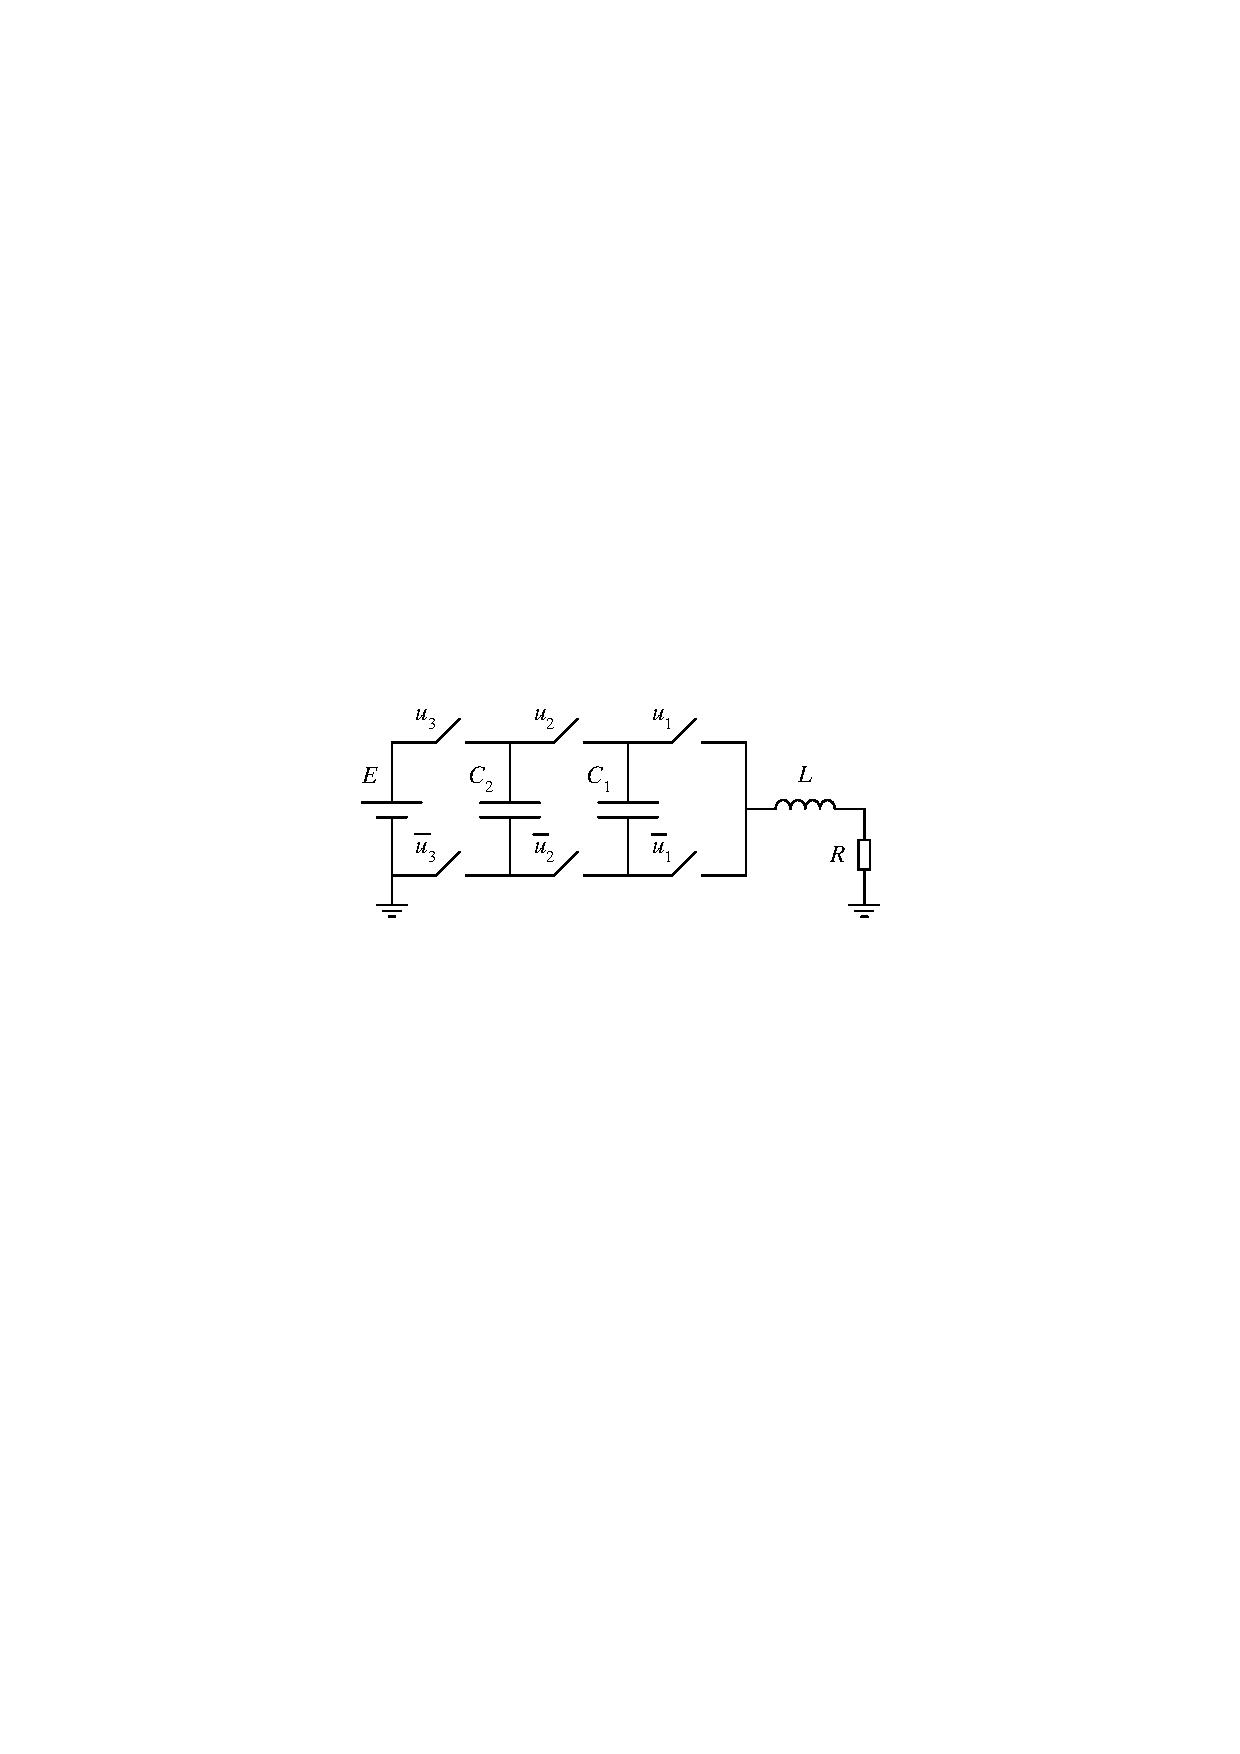
\includegraphics[scale=1]{CircuitDiagram.pdf}
  \end{center}
  \caption{Circuit topology.}
\end{figure}

A common method to operate the converter is the so-called Phase-Shifted Modulation (PSM) scheme \cite[p. 74-77]{Saenz:2014}. For a $p$-cell converter, the PSM scheme employs $p$ triangular modulation signals $s_1(t), s_2(t), \ldots, s_p(t)$, which oscillate in the 0 - 1 range with frequency $f = 1/T$ and $2 \pi / p$  phase shifts, as illustrated in Figure \ref{fig:PSM} for $p = 3$. Signal $s_i(t)$ is associated to the $u_i(t)$ switch command in the converter, so that
%
\begin{equation}
  u_i(t) = \left\{
  \begin{array}{l}
    0 \,,\; s_i(t) \geq \alpha \\[6pt]
    1 \,,\; s_i(t) < \alpha
  \end{array}
  \right.
\end{equation}
%
where $\alpha = v_{out} / E  \in [0, 1]$ is the desired voltage fraction at the converter output. As can be seen from Fig. \ref{fig:PSM}, the ``on" and "off" times are the same for all switch commands, namely:

\begin{equation}
  \Delta t_{on} = \alpha T \,, \; \Delta t_{off} = (1 - \alpha) T
\end{equation}

\begin{figure}[h]
  \label{fig:PSM}
  \begin{center}
    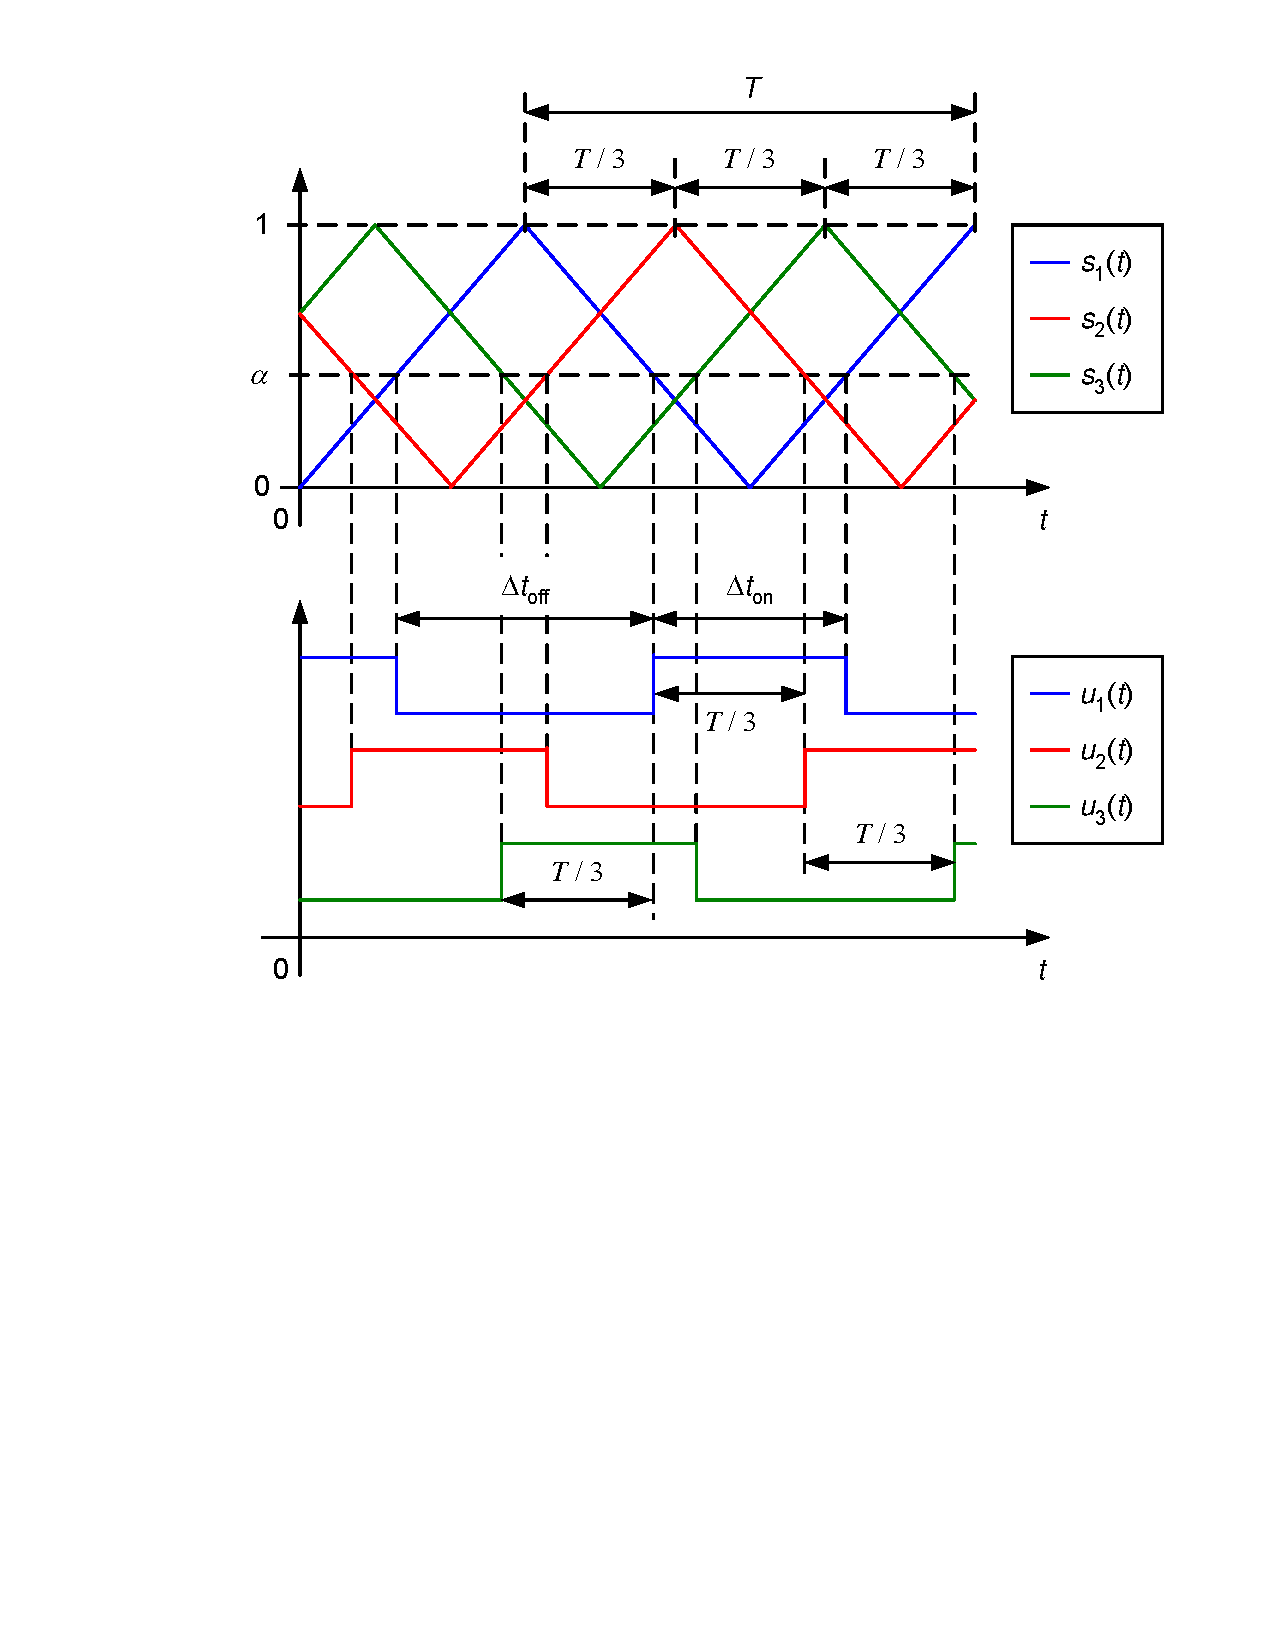
\includegraphics[scale=0.75]{PhaseShiftModulation.pdf}
  \end{center}
  \caption{Phase-shifted modulation scheme for the three-cell converter.}
\end{figure}



\begin{figure}[h]
  \label{fig:Schematics}
  \begin{center}
    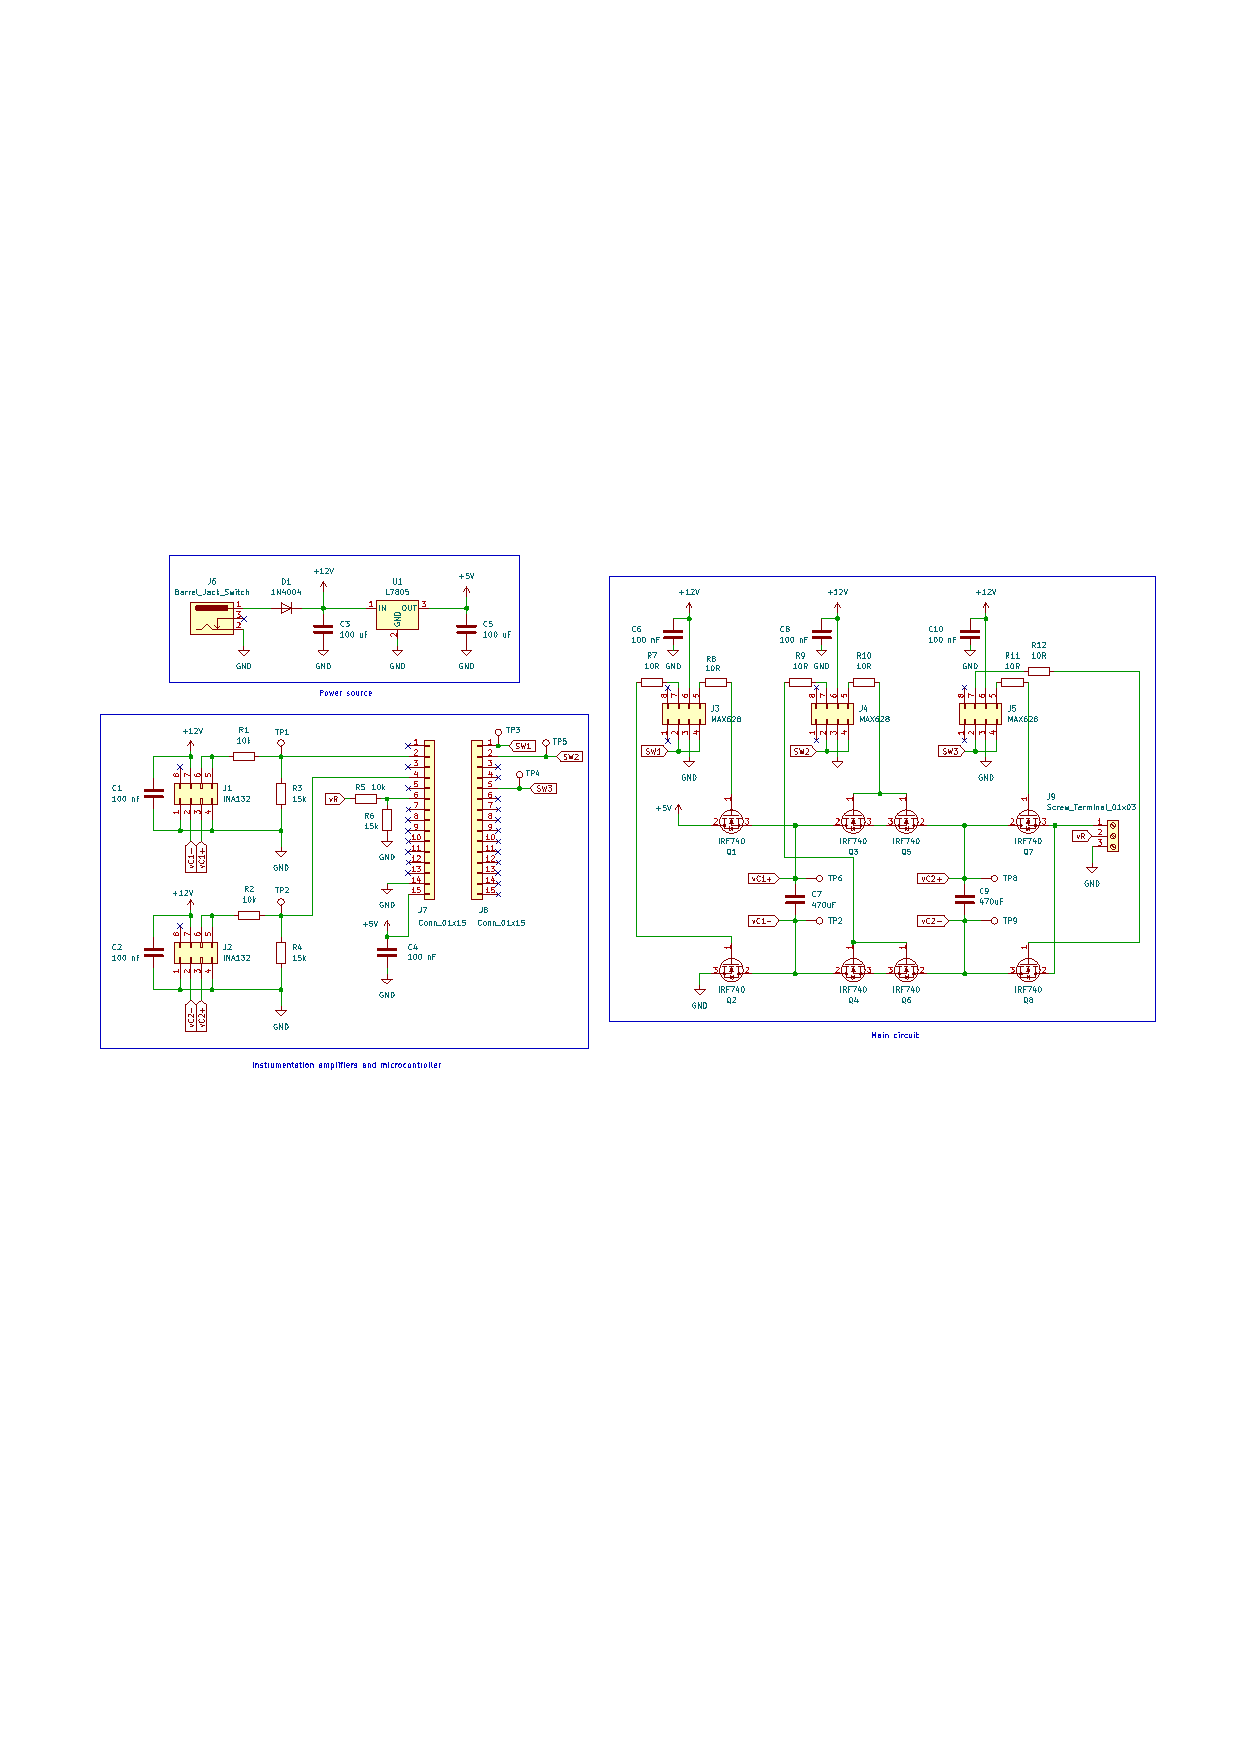
\includegraphics[scale=1]{Schematics.pdf}
  \end{center}
  \caption{Circuit schematics.}
\end{figure}


\newpage

\section*{\textit{Design files}}
% The  complete  design  files  must  be  either  uploaded  to  an  approved  online  repository,  uploaded  at the  time  of  submission  on  the  online  Editorial  Manager  submission  interface  as  supplementary materials [CAD files, videos,. . . ], or included in the body of the manuscript [e.g.  figures].  The three approved  online  repositories  are  Mendeley  Data,  the  Open  Science  Framework,  and  Zenodo. See repository instructions: https://doi.org/10.5281/zenodo.3346799

% Design files should be in preferred format for making modifications. See OSHWA’s open-source definition for details: https://www.oshwa.org/definition/

\textit{Your design files should be editable - see \href{https://www.oshwa.org/definition/}{OSHWA’s open source definition of ‘Documentation’} for further details. You must then either:}
\begin{itemize}
  \item[$\bullet$]{\it Upload your design files to one of the three approved online repositories - \href{https://data.mendeley.com/}{Mendeley Data} (\href{https://doi.org/10.5281/zenodo.3346799}{instructions}), the \href{https://osf.io/}{Open Science Framework} (\href{https://osf.io/wgk7q/wiki/home/}{instructions}) or \href{https://zenodo.org/}{Zenodo} (\href{https://doi.org/10.5281/zenodo.3346799}{instructions}). We recommend this option as the repositories support versioning of files.}
  \item[$\bullet$]{\it Upload your design files as supplementary materials (e.g., CAD files, videos…) to Hardware X’s online editorial system when you submit your manuscript.}
  \item[$\bullet$]{\it Include your design files in the body of the manuscript (e.g., as figures).}
\end{itemize}

%
%\textit{The complete design files must be either uploaded to an approved online repository, uploaded at the time of submission on the online \href{https://editorialmanager.com/ohx/}{Editorial Manager} submission interface as supplementary materials [CAD files, videos,\dots], or included in the body of the manuscript [e.g. figures]. The three approved online repositories are \href{https://data.mendeley.com/}{Mendeley Data}, the \href{http://osf.io}{Open Science Framework}, and \href{https://zenodo.org/}{Zenodo}. See repository instructions \href{https://doi.org/10.5281/zenodo.3346799}{here}. Design files should be in preferred format for making modifications. See \href{https://www.oshwa.org/definition/}{OSHWA’s open-source definition} for details.}
%\begin{itemize}
\vskip 0.1 cm
\noindent
\textit{\underline{CAD files:} You are encouraged to use free and open source software packages for creating the files. For CAD files, \href{http://www.openscad.org/}{OpenSCAD}, \href{http://www.freecadweb.org/}{FreeCAD}, or \href{https://www.blender.org/}{Blender} are encouraged, but, if these are not available, we accept source files from proprietary CAD packages, such as Autocad or Solidworks, and other drawing packages.}
\vskip 0.1 cm
\noindent
\textit{\underline{3D printing:} Supplementary files that facilitate digital replication of the devices are encouraged;  for example, STL files for 3D printing components. We recommend uploading CAD files to the \href{http://3dprint.nih.gov/}{\underline{NIH 3D Print Exchange}} as Custom Labware and then entering the link here.}
\vskip 0.1 cm
\noindent
\textit{\underline{Electronics:} PCB layouts and other electronics design files can be uploaded to the \href{http://www.ohwr.org/}{\underline{Open Hardware Repository}} or other repositories or as supplementary materials.}
\vskip 0.1 cm
\noindent
\textit{\underline{Software and firmware:} All software files used in the design and operation of the hardware should be included in the repository. Provide a description of the software and firmware and use extensive comments in the code.}

\section{Design files summary}
\textit{Complete a separate row for each design file associated with your hardware (including the primary design files). Any empty rows should be deleted.}
% Please include a summary of all design files for your hardware by filling rows of the table below
\vskip 0.1cm
\tabulinesep=1ex
\begin{tabu} to \linewidth {|X|X|X[1.5,1]|X[1.5,1]|}
  \hline
  \textbf{Design filename}            & \textbf{File type}                      & \textbf{Open source license}                                                                                                     & \textbf{Location of the file}                                                                   \\\hline
  %Insert design files
  \textit{For example: Design file 1} & \textit{e.g. CAD file, figures, videos} & \textit{All designs must be submitted under an open hardware license. Enter the corresponding open source license for the file.} & \textit{Either enter the URL for the repository or the sentence: "Available with the article".} \\\hline
  \dots                               & \dots                                   & \dots                                                                                                                            & \dots                                                                                           \\\hline
  \dots                               & \dots                                   & \dots                                                                                                                            & \dots                                                                                           \\\hline
  % Design file 3 & File type & License & Link \\\hline
\end{tabu}


% For each design file listed in the summary above, include a short description of the file below (one or two sentences)
\vskip 0.3cm
\noindent
\textit{For each design file listed in the summary table above, include a short description of the file below (just one or two sentences per design file).}

%\section*{\textit{Bill of materials}}
% For a complex Bill of Materials, the complete Bill of Materials (editable spreadsheet file e.g., ODS file type or PDF file) can be uploaded in an open access online location such as the Open Science Framework repository. Include the link here. Alternatively, the Bill of Materials can be uploaded at the time of submission on the online Elsevier submission interface as supplementary material.

% > To make it easy to tell which item in the Bill of Materials corresponds to which component in your design file(s), use matching designators in both places, or otherwise explain the correspondence.

% > For material type, select from: Metal, semi-conductor, ceramic, polymer, biomaterial, organic, inorganic, composite, nanomaterial, semiconductor, non-specific, or other  


\section{Bill of materials summary}
\tabulinesep=1ex
\noindent

\textcolor{red}{Preencher Google Sheet em}

\textcolor{blue}{
  https://docs.google.com/spreadsheets/d/14c4qT01m3tA2rBspwJqqd35RiecyckPLIuiIuWBo2DA/edit?usp=sharing}

% % defining url's
% \urldef{\aliexpressurl}\url{https://www.aliexpress.com/item/1005006844873587.html?spm=a2g0o.productlist.main.9.5c8b640crrwiUa&algo_pvid=3916fe28-c01d-45b7-8975-0dc065f15c56&algo_exp_id=3916fe28-c01d-45b7-8975-0dc065f15c56-8&pdp_ext_f=%7B%22order%22%3A%22243%22%2C%22eval%22%3A%221%22%7D&pdp_npi=4%40dis%21USD%212.23%212.23%21%21%2115.84%2115.84%21%402103277f17535278073698102e9b73%2112000038492445322%21sea%21BR%213505867280%21X&curPageLogUid=ECUlwNYTI6XL&utparam-url=scene%3Asearch%7Cquery_from%3A}
% \urldef{\mouserurl}\url{https://www.mouser.com/ProductDetail/Texas-Instruments/INA132U-2K5?qs=VBduBm9rCJQmjzz%2FewsuqQ%3D%3D}

% \begin{tabu} to \linewidth {|X[1.1,1]|X|X[0.6,1]|X[0.8,1]|X|X|X[1.1,1]|}
% %\begin{tabular}{|c|c|c|c|c|c|c|}
% \hline
% \textbf{Designator} & \textbf{Component} & \textbf{Number} & \textbf{Cost per unit - currency} & \textbf{Total cost - currency} & \textbf{Source of materials} & \textbf{Material type} \\\hline

% %Insert items here
% \textit{If possible, use the same designator here as you use in the associated design file. If that’s not possible, you will need to explain the relationship between the two.} & \textit{Name of Component 1} & \textit{Number of units} & \textit{Cost per unit and the currency used} & \textit{Total cost and the currency used} & \textit{If possible, include a direct link to a webpage where the component can be purchased } & \textit{Select from:
% \vskip 0.1cm
% %\begin{itemize}
% -Metal
% \vskip 0.1cm
% -Semi-conductor
% \vskip 0.1cm
% -Ceramic
% \vskip 0.1cm
% -Polymer
% \vskip 0.1cm
% -Biomaterial
% \vskip 0.1cm
% -Organic
% \vskip 0.1cm
% -Inorganic
% \vskip 0.1cm
% -Composite
% \vskip 0.1cm
% -Nanomaterial
% \vskip 0.1cm
% -Semiconductor
% \vskip 0.1cm
% -Non-specific
% \vskip 0.1cm
% -Other 
% %\end{itemize}
% } \\\hline
% R1, R2, R3, R4, R5, R6 & 10 $\Omega$ Resistor & 6 & \dots & \dots & \dots & Electronic \\\hline

% \dots & Borne & 4 & \dots & \dots & \dots & \dots \\\hline

% \dots & M3 screw and nut & 4 & \dots & \dots & \dots & \dots \\\hline

% \dots & Rubber pad & 4 & \dots & \dots & \dots & \dots \\\hline

% \dots & Coil 100 mH & 1 & \dots & \dots & \dots & \dots \\\hline

% \dots & Screw socket 3 connectors & 1 & \dots & \dots & \dots & \dots \\\hline

% \dots & 3 pin DIP socket (optional) & 8 & \dots & \dots & \dots & \dots \\\hline

% \dots & Female pin bar & 1 & \dots & \dots & \dots & \dots \\\hline

% \dots & DIP-8 socket & 5 & \dots & \dots & \dots & \dots \\\hline

% \dots & 100 nF ceramic capacitor & 3 & \dots & \dots & \dots & \dots \\\hline

% \dots & 100 $\mu$ F / 35 V electrolitic capacitor & 3 & \dots & \dots & \dots & \dots \\\hline

% \dots & ESP-32 & 1 & \dots & \dots & \dots & \dots \\\hline

% \dots & TSC-428 driver & 3 & \dots & \dots & \dots & \dots \\\hline

% \dots & IRF 740 n-channel mosfet & 8 & US\$2.28 (10 pieces) & US\$2.28 & \aliexpressurl & \dots \\\hline

% \dots & 22 $\Omega$ / 1 W resistor & \dots & \dots & \dots & \dots & \dots \\\hline

% \dots & 470 $\mu$F / 35 V electrolitic capacitor & \dots & \dots & \dots & \dots & \dots \\\hline

% \dots & INA-132 instrumentation amplifier & 2 & US\$3.60 & US\$7.20 \dots & \mouserurl & \dots \\\hline

% \dots & 10 cm x 10 cm Double-sided copper board & 1 & \dots & \dots & \dots & \dots \\\hline

% % Designator 3 & Name of Component 2 & Number of units & Cost per unit & Total cost & Source of materials & Material type \\\hline
% \end{tabu}\\
% \vskip 0.2cm
% %\end{tabular}
% \noindent
% \textit{You can use this space for any additional descriptions of the materials used.}

\section{Build instructions}
%Provide detailed, step by step instructions for the construction of the reported hardware include all necessary information for reproducing the submitted hardware.
% > Explain and, when possible, characterize design decisions. Including design alternatives if they exist. 
% > Use visual instructions such as schematics, images, and videos. 
% > Clearly reference design files and component parts described in the Design File Summary and Bill of Materials. 
% >Highlight potential safety concerns that may arise

\textit{Provide detailed, step-by-step construction instructions for the submitted hardware:
  \begin{itemize}
    \item[$\bullet$]Include all necessary information for reproducing it.
    \item[$\bullet$]Explain and (when possible) characterize design decisions. Include any design alternatives you created.
    \item[$\bullet$]Use visual instructions such as schematics, images and videos.
    \item[$\bullet$]Clearly reference design files and component parts described in the \textbf{Design file summary} and the \textbf {Bill of materials summary}.
    \item[$\bullet$]Highlight any potential safety concerns.
  \end{itemize}}

\begin{figure}[h]
  \label{fig:PCB}
  \begin{center}
    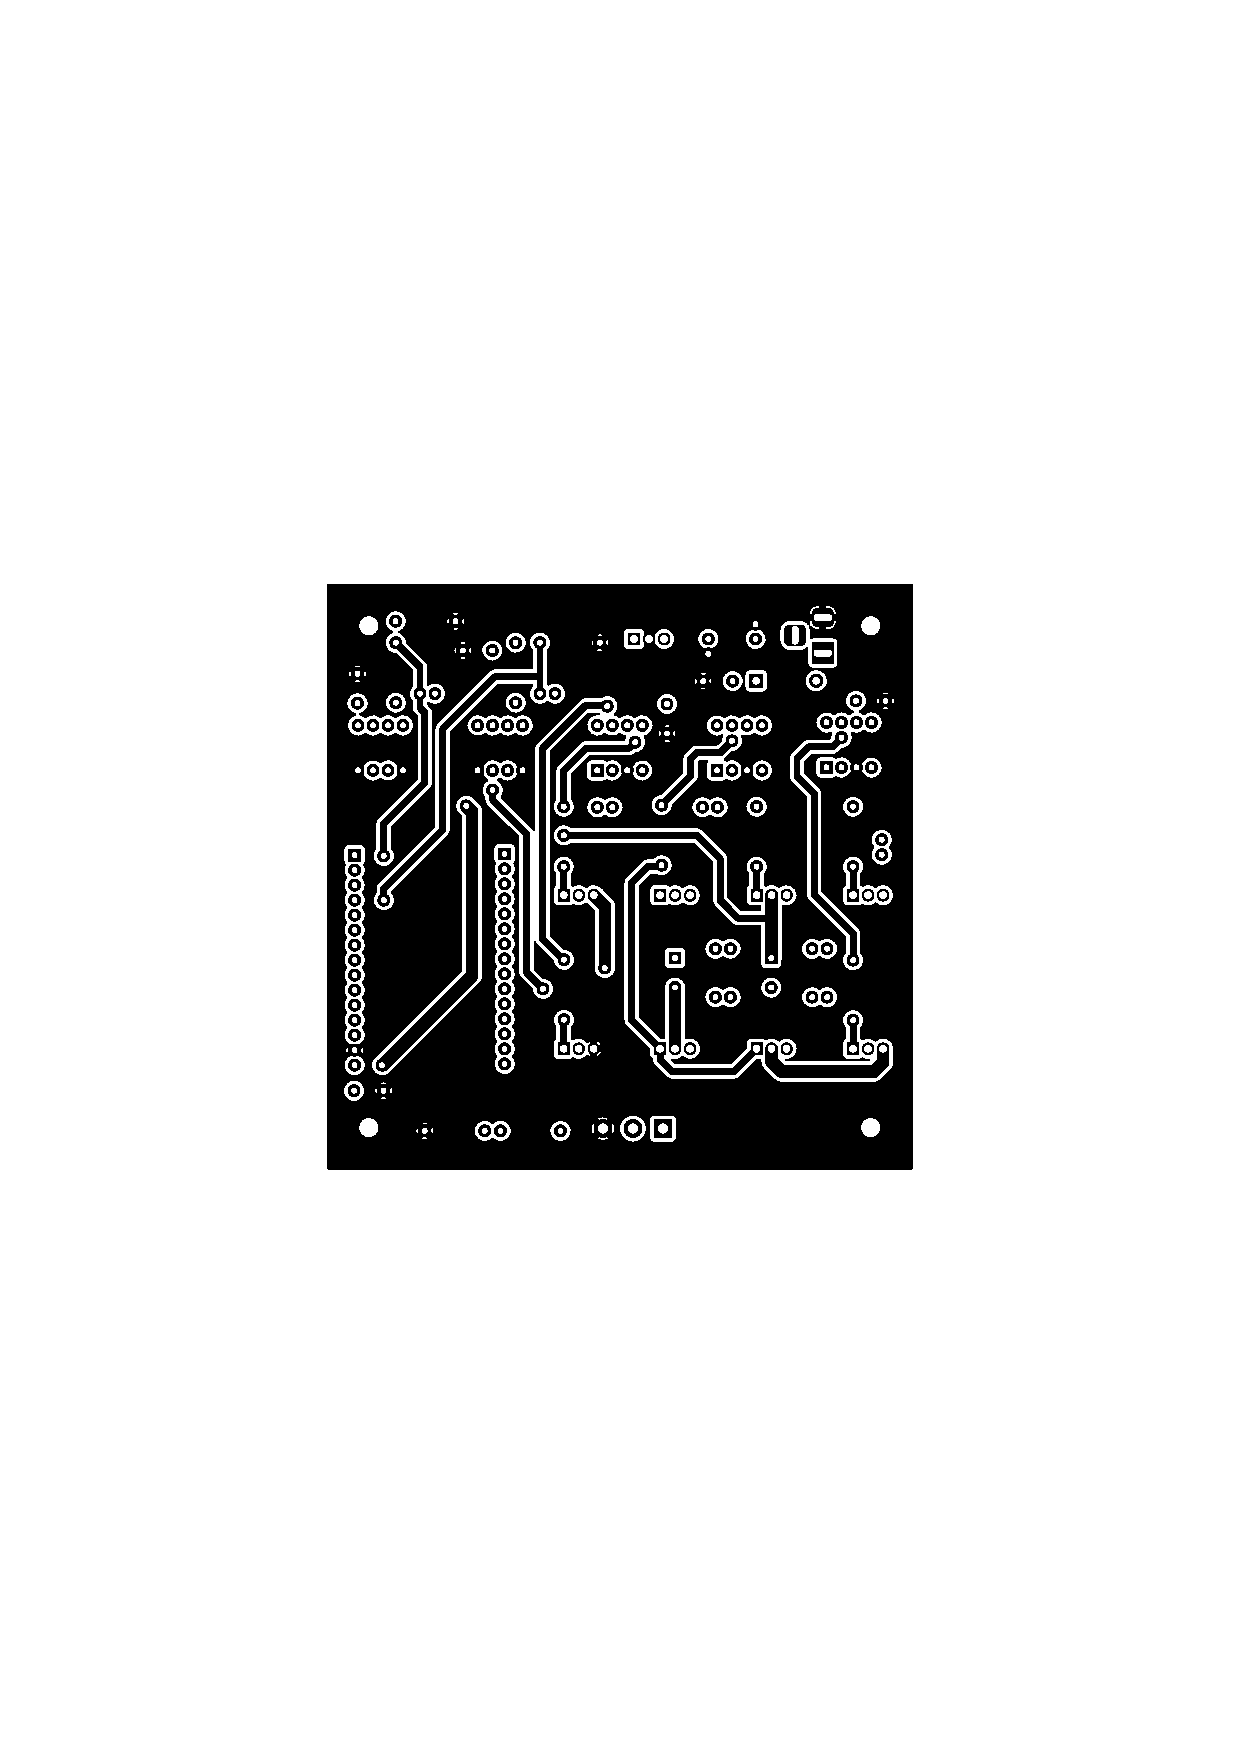
\includegraphics[scale=0.7]{Front.pdf}
    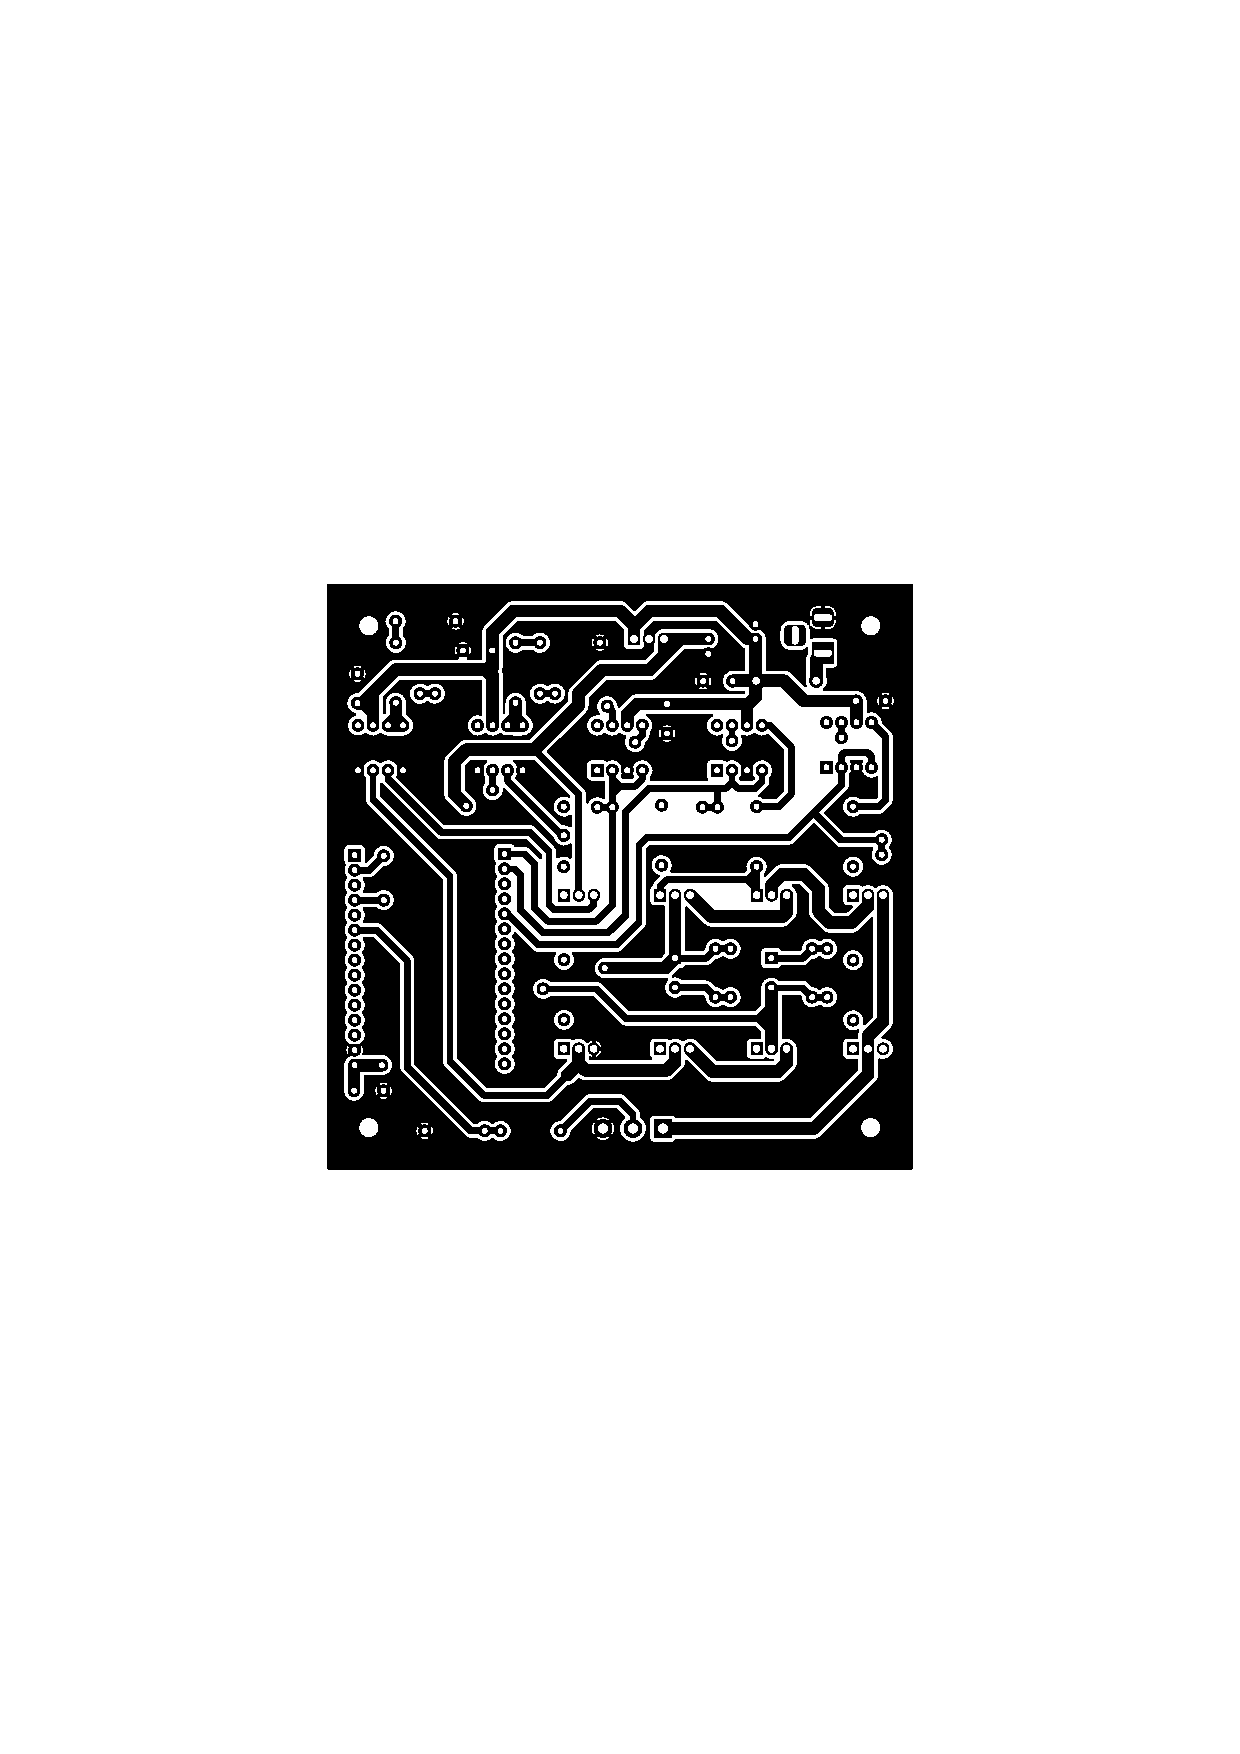
\includegraphics[scale=0.7]{Back.pdf}
  \end{center}
  \caption{PCB layout: Front (left) and Back (right).}
\end{figure}

\begin{figure}[h]
  \label{fig:Photo}
  \begin{center}
    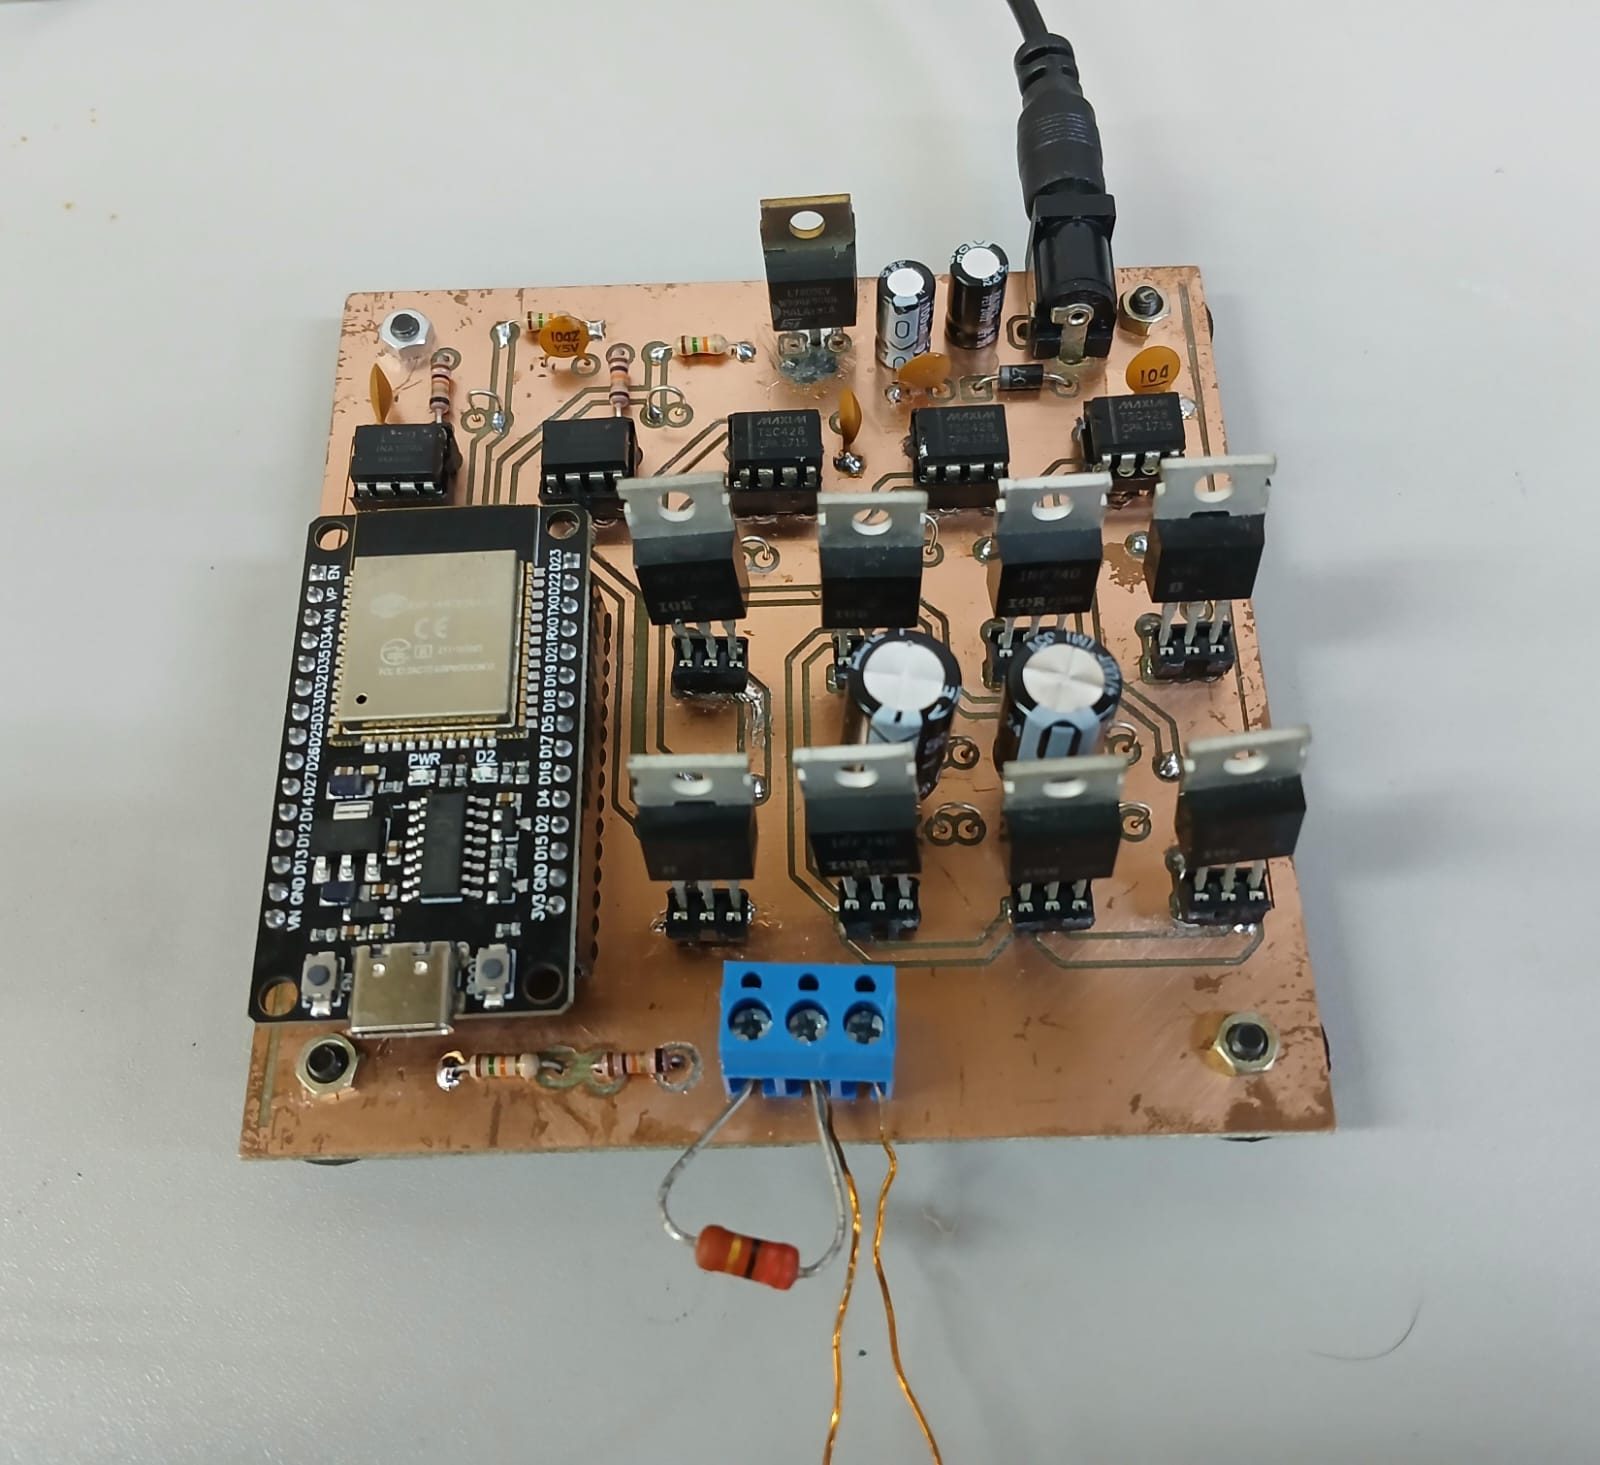
\includegraphics[scale=0.25]{DevicePhoto.jpeg}
  \end{center}
  \caption{Photo of the device. The $10 \Omega$ resistors R1, R2, $\ldots$, R6 are soldered on the bottom.}
\end{figure}


\section{Software Architecture and Implementation}

The software system is designed as a platform for real-time control and experimental monitoring, 
consisting of a high-precision firmware engine for the ESP32 and a responsive web interface. 
The integration leverages the Bluetooth Low Energy (BLE) protocol to establish the link between 
the embedded hardware and the user's browser.

\section{Firmware Design and Hardware-Level Optimization}

The ESP32 firmware is developed using the ESP-IDF framework to fine control the hardware's dual-core 
capabilities and real-time features. To ensure deterministic performance, specific hardware-level 
configurations are defined in the project using the \textbf{idf menuconfig}.

\begin{itemize}
	\item \textbf{CPU Frequency:} The system is locked at \textbf{240 MHz} to provide the maximum
	      timing resolution for the signal generation loops.

	\item \textbf{Dual-Core Execution:} The ESP32's dual-core capability is used to separate
	      time-critical signal generation from non-deterministic communication.

	\item \textbf{Watchdog Management:} To prevent system resets during continuous signal
	      generation, the Task Watchdog Timer (TWDT) is explicitly disabled for \textbf{Core 1}
	      (\verb|CONFIG_ESP_TASK_WDT_CHECK_IDLE_TASK_CPU1|). This allows the signal task to occupy the
	      CPU cycles without yielding.
\end{itemize}

\subsection{The Real-Time Signal Engine}

The implementation of the signal engine in \verb|signal_controller.cpp| prioritizes speed and timing 
consistency. Rather than relying on standard high-level APIs, the engine utilizes atomic register 
manipulation to perform simultaneous GPIO updates. Key highlights of this implementation include:

\begin{itemize}
\item \textbf{Atomic Switching for Precision:} To protect the voltage converter from 
"shoot-through" currents, the firmware enforces a precise dead-time interval during switching 
transitions. As shown in Listing \ref{lst:switching}, the system utilizes atomic registers 
(\verb|GPIO.out_w1tc| and \verb|GPIO.out_w1ts|) to pull pins low immediately before applying a 
sub-microsecond delay calibrated to the 240 MHz clock. 

\begin{lstlisting}[caption={Atomic Switching and Dead-Time Implementation}, label={lst:switching}] 
// From signal_controller.cpp 
if (clear_mask) { 
    GPIO.out_w1tc = clear_mask; // Atomic clear (Dead Time start)

    uint32_t delay_val = is_rising ? g_cycle_us_delay_up : g_cycle_us_delay_down;
    helper_delay_cycles(delay_val); 

    GPIO.out_w1ts = set_mask;   // Atomic set (Dead Time end)
} 
\end{lstlisting}

	\item \textbf{Double-Buffering Logic:} To allow dynamic parameter updates without halting the 
		hardware output, the firmware maintains an "active" and "inactive" dataset. While 
		\textbf{Core 1} drives the converter using the active set, \textbf{Core 0} parses new 
		commands into the inactive set.

	\item \textbf{Seamless Synchnization:} As illustrated in Listing \ref{lst:buffer}, a synchronization flag 
		(\verb|g_ds_update_pending|) triggers a pointer swap at the start of the next signal cycle, 
		ensuring a glitch-free transition between experimental patterns. 
		

\begin{lstlisting}[caption={Double-Buffer Synchronization Mechanism}, label={lst:buffer}] 
// From signal_controller.cpp 
if (g_ds_update_pending) { 
	if (g_active_set == SignalSet::SET_A) {
		dataset = &g_dataset_b; 
		g_active_set = SignalSet::SET_B; 
	} else { 
		dataset = &g_dataset_a; 
		g_active_set = SignalSet::SET_A; 
	} 

	g_ds_update_pending = false; 
} 
\end{lstlisting}
\end{itemize}

\subsection{Data Acquisition and Calibration}

Real-time monitoring is achieved through a dedicated task that samples the voltages across the 
converter's flying capacitors and the load. Given the non-linear response of the ESP32's 
analog-to-digital converter (ADC), the system incorporates a calibration layer using eFuse-stored 
factory constants and a custom \textbf{Lookup Table (LUT)}.

\begin{lstlisting}[caption={Linear Interpolation Calibration Function}, label={lst:calib}] 
// From helper_analog.cpp 

float esp32_calibration(float value) {
    for (int i = 0; i < calib_numel - 1; ++i) {
        if (value >= calib_from[i] && value <= calib_from[i + 1]) {
            float x1 = calib_from[i];
            float y1 = calib_to[i];
            float x2 = calib_from[i + 1];
            float y2 = calib_to[i + 1];
            return y1 + (value - x1) * (y2 - y1) / (x2 - x1);
        }
    }
    return calib_to[calib_numel - 1];
}
\end{lstlisting}

This calibration utilizes linear interpolation between measured points (Listing \ref{lst:calib}) 
to map raw ADC counts to accurate physical voltages. These values are then packaged into BLE 
notifications for real-time visualization on the web interface.

\subsubsection{Configuration and Control Logic}

The following tables (\ref{tab:system-config} and \ref{tab:ble-commands}) summarize the critical settings and commands required to reproduce the 
system's performance and manage experimental parameters.

\begin{table}[htbp]
	\centering
	\caption{Hardware-Level Firmware Build Configurations}
	\label{tab:system-config}
	\begin{tabular}{llp{8cm}}
		\toprule
		\textbf{Configuration Parameter} & \textbf{Value} & \textbf{Function}                                                        \\
		\addlinespace
		CPU Frequency                    & 240 MHz        & Maximizes timing resolution for helper\_delay\_cycles and system delays. \\
		\addlinespace
		FreeRTOS Cores                   & 2 Cores        & Enables task pinning for core isolation between Signal and BLE domains.  \\
		\addlinespace
		Task Watchdog (Core 1)           & Disabled       & Prevents system reset while the signal task maintains CPU occupancy.     \\
		\addlinespace
		ADC Calibration                  & LUT            & Necessary to correct native non-linearities for analog data acquisition. \\
		\addlinespace
		BLE Stack                        & Bluedroid      & Provides the GATT server infrastructure for remote control.              \\
		\bottomrule
	\end{tabular}
\end{table}


\begin{table}[htbp]
	\centering
	\caption{BLE Communation and Command Router}
	\label{tab:ble-commands}
	\begin{tabular}{llp{8cm}}
		\toprule
		\textbf{Command String} & \textbf{Description} & \textbf{Operational Effect}                                                \\
		\addlinespace
		\verb|SIGNAL:{t;m}|     & Raw Vector Update    & Updates the timing (t) and mode (m) vectors in the inactive dataset.       \\
		\addlinespace
		\verb|SET_ALPHA:x|      & Automatic PSM        & Calculates a Phase-Shifted Modulation pattern for a specific duty cycle x. \\
		\addlinespace
		\verb|START / STOP|     & State Control        & Toggles the signal generation loop between running and idle states.        \\
		\addlinespace
		\verb|STATUS|           & System Metrics       & "Returns current cycle counts, active datasets, and hardware statuses."    \\
		\bottomrule
	\end{tabular}
\end{table}



















\vspace*{20cm}
IK BEN HIER


\subsection{Part 2: The Web Control Interface}

This is the user interface of the system for controlling the ESP32.
It is build with web technologies to run in any browser that supports
Web Bluetooth.

\subsubsection{Core Capabilities}

\begin{itemize}
	\item \textbf{React \& TypeScript:} The application is build using React, a popular
	      JavaScript library for building user interfaces, and TypeScript, which adds static
	      typing to JavaScript. This combination allow a code that is both portable and
	      maintainable.
	\item \textbf{Web Bluetooth API:} The Web Bluetooth API is a browser standard that
	      exposes Bluetooth functionality to JavaScript, allowing the application to
	      \subitem \textbf{Scan} for nearby BLE devices
	      \subitem \textbf{Connect} to a selected device (ESP32)
	      \subitem \textbf{Discover} its services and characteristics
	      \subitem \textbf{Write} data to characteristics (to send commands)
	      \subitem \textbf{Subscribe} to notifications from characteristic (to receive sensor data)
\end{itemize}

This eliminates the need for any native software, drivers, or browser plugins. The entire control
system runs directly in the browser.


\begin{lstlisting}[caption={Bluetooth connect\_device}]
// from bluetooth.ts

export async function connect_device() {
    try {
        let navigatorObject: any = window.navigator;

        // Open the device picker dialog, filtering for our specific service
        g_bluetoothDevice = await navigatorObject.bluetooth.requestDevice({
            filters: [{ services: [SERVICE_UUID] }],
        });

        // Connect to the device's GATT server
        g_gattServer = await g_bluetoothDevice.gatt.connect();

        // Get the service we're interested in
        const service = await g_gattServer.getPrimaryService(SERVICE_UUID);

        // Get the characteristic we'll use for reading/writing data
        g_characteristic = await service.getCharacteristic(CHARACTERISTIC_UUID);

    } catch (error: any) {
        // Handle any errors during the connection process
    }
}
\end{lstlisting}

\subsection{Web Interface}

The web interface is built with React.js to provide an easy user experience.
This interface serves as the primary connection point between the user and the hardware,
linking directly to the ESP32 microcontroller via Bluetooth Low Energy (BLE).

From the web application (Figure \ref{fig:sw_web_interface}), users can easily send string commands to the device, as well as trigger automated
sequences for common experimental procedures. A key function of the interface is its ability to perform
on-the-fly computations to generate the control signals needed for the power switches. It also
receives and processes data from the ESP32's BLE connection, specifically the analog measurements from
the circuit. The received data is then visually represented in a real-time chart, allowing for immediate
analysis of the circuit's performance.


\begin{figure}[h!]
	\centering
	
\includegraphics[width=140mm]{images/hw_esp32_pins.pdf}
	\caption{ESP32 Digital and Analog mapping}
	\label{fig:sw_esp_pins}
\end{figure}


\begin{figure}[h!]
	\centering
	
\includegraphics[width=140mm]{images/sw_web_interface.pdf}
	\caption{Web Interface to connect and control the ESP32.}
	\label{fig:sw_web_interface}
\end{figure}

The web interface provides single-page application for interacting
with the hardware in real-time. It connects to the ESP32 via Bluetooth Low Energy (BLE) and serves as
a command center for controlling the circuit and analyzing its performance. The following are the key
features of the interface:

\begin{itemize}
	\item \textbf{1. Connect/Disconnect:} Establish or terminate a BLE connection to the ESP32.
	\item \textbf{2. Status command:} Sends the command to get the status of the ESP32 program.
	\item \textbf{3. copy:} Copy the logged data to use in plot or analysis.
	\item \textbf{4. Clear Data:} Clear the logged data.
	\item \textbf{5. $<img>$:} When clicked on the image, the web interface then shows the schematics of the circuit and the connections of the
	      ESP32. This is used as a reference while connecting the circuit.

	\item \textbf{6. Enter command:} Send raw command to ESP32 through BLE.

	\item \textbf{7. SEND:} Send the raw command to the ESP32.

	\item \textbf{8. START:} Commands the ESP32 to start reproducing the signal created.
	\item \textbf{9. STOP (Low):} Commands the ESP32 to set all digital outputs to LOW (0).
	\item \textbf{10. HIGH:} Commands the ESP32 to set all digital outputs to HIGH (1).

	\item \textbf{11. Alpha:} Input tor selecting the alpha value to compute the signal.
	\item \textbf{12. Time:} Time vector in micro seconds ($\mu s$)

	      each element is a amount of $\mu s$ that the mode is going to be executed.

	\item \textbf{13. Mode:} Mode vector for the digital output

	      the mode is the decimal representation of the three digital outputs.
	      The digital output is set to send value to D4, D5 and D6 (figure \ref{fig:sw_esp_pins}).

	      When 13.1 is clicked then the interface shows the decomposed values for each channel D4, D5 and D6.

	      The example in figure \ref{fig:sw_web_interface}, generates the digital signals
	      d4: [0, 0, 0, 1, 1, 1], d5: [0, 1, 1, 1, 0, 0], d6: [1, 1, 0, 0, 0, 1] as result of the
		  signal generated by the Alpha of 0.5.

	      The signal is represented in Figure \ref{fig:sw_signal}.

	      \begin{figure}[h!]
		      \centering
		      
\includegraphics[width=140mm]{images/sw_signal.pdf}
		      \caption{Signal for $\alpha$ of 0.4}
		      \label{fig:sw_signal}
	      \end{figure}

	\item \textbf{13.1. UPLOAD:} Shows the Binary representation of the signal modes.

	\item \textbf{14. UPLOAD:} Send the Signal (Time and Mode) to the ESP32.

	\item \textbf{15. Chart Toggle:} Collapses or expand the Chart to show the voltage reading via BLE.
	\item \textbf{16. Advanced Menu Toggle:} Collapses or expand the menu with pre-configured facility commands to send messages via BLE.
	\item \textbf{17. Monitor Chart:} When `Start Listening` is active, then the Monitor chart shows the values of the analog readings from the ESP32.
	\item \textbf{18. System Log:} Displays the log messages from the ESP32.
	\item \textbf{19. Advanced Menu:} Collection of buttons with preconfigured commands.
\end{itemize}

The system's behavior is described by a state diagram in Figure \ref{fig:state_diagram} that shows the
Overall System Flow, which transitions from an initial Setup phase into two main concurrent processes: BLE Task States and Signal Task States.

The BLE (Bluetooth Low Energy) task handles wireless communication
and sensor data, cycling through states such as BLE\_IDLE (when no operations are active), ANALOG\_READING
(when it's actively reading sensor data), and SIGNAL\_READING (when it's processing new signal information).

Concurrently, the Signal task manages the output signals, operating in states like IDLE (with no signals
generated), HIGH\_ALL (where all outputs are forced high), and SIGNAL\_RUN (for active signal pattern
generation). This dual-task structure allows the system to manage sensor inputs and signal outputs independently.

\begin{figure}[h]
	\centering
	
\includegraphics[scale=0.5]{images/sw_state_machine.png}
	\caption{State Diagram of the SW Operation Modes}
	\label{fig:state_diagram}
\end{figure}


\section{Operation instructions}
%Provide detailed instructions for the safe and proper operation of the hardware. 
%> Step-by-step operational instructions for operating the hardware. 
%> Use visual instructions as necessary. 
%> Highlight potential safety hazards.

\textit{Provide detailed, step-by-step instructions for the safe and proper operation of the hardware.
  \begin{itemize}
    \item[$\bullet$]Use visual instructions, as necessary.
    \item[$\bullet$]Highlight any potential safety hazards.
  \end{itemize}}

\section{Validation and characterization}
%Demonstrate the operation of the hardware and characterize its performance over relevant critical metrics
%> Demonstrate the use of the hardware for a relevant use case. 
%> If possible, characterize performance of the hardware over operational parameters. 
%> Create a bulleted list that describes the capabilities (and limitations) of the hardware. For example consider descriptions of load, operation time, spin speed, coefficient of variation, accuracy, precision and etc. 

\textit{Demonstrate the operation of the hardware and characterize its performance for a specific scientific application.
  \begin{itemize}
    \item[$\bullet$]Highlight a relevant use case.
    \item[$\bullet$]If possible, characterize performance of the hardware over operational parameters.
    \item[$\bullet$]Create a bulleted list describing the capabilities (and limitations) of the hardware. For example, load and operation time, spin speed, coefficient of variation, accuracy, precision, etc.
  \end{itemize}}

Figure \ref{fig:Commands} presents the switch commands $u_1(t)$, $u_2(t)$, $u_3(t)$ for $\alpha = 0.3$. The waveforms were acquired at the test points TP3, TP4, TP5 using a  Tektronix TDS 2004B oscilloscope.

\begin{figure}[h]
  \label{fig:Commands}
  \begin{center}
    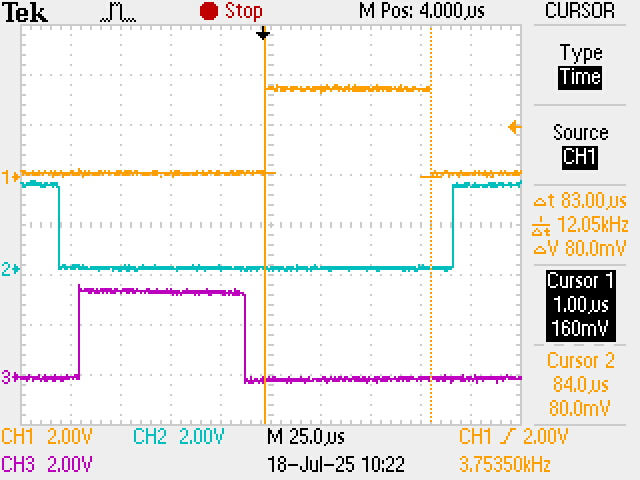
\includegraphics[scale=1]{Ton.jpg}
    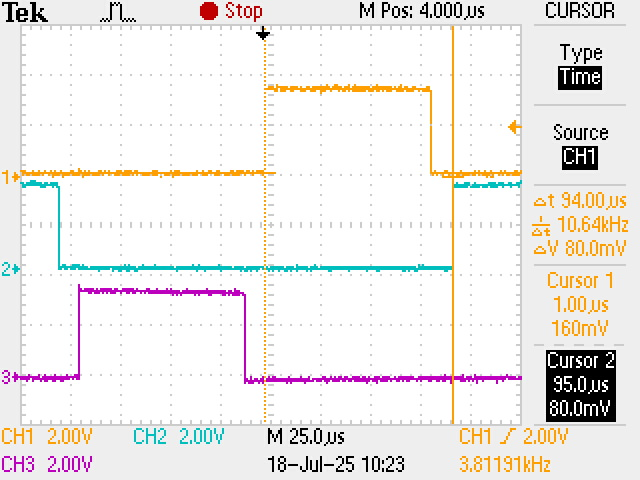
\includegraphics[scale=1]{DeltaT_12.jpg}
    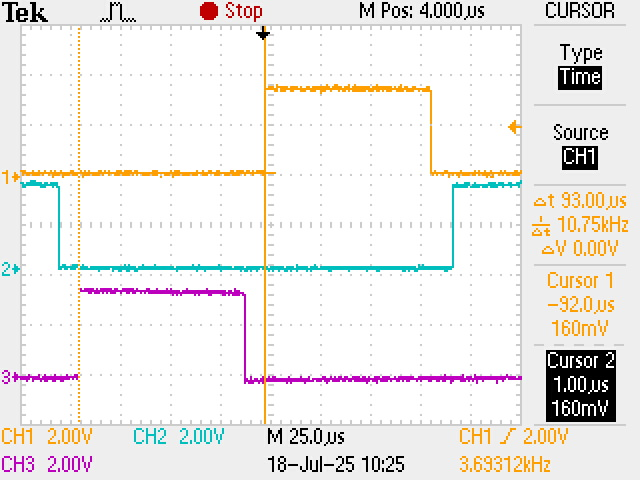
\includegraphics[scale=1]{DeltaT_31.jpg}
  \end{center}
  \caption{Commands $u_1(t)$, $u_2(t)$, $u_3(t)$ with $\alpha = 0.3$ and $T = $ \textcolor{red}{???} (a) $\Delta T_{on} = 83 \mu$s.}
\end{figure}




Note that $T = 1/(3.75 \text{ kHz} = 0.27$ ms. \textcolor{red}{Confirmar valores usados no código.} \\

\noindent
\textbf{Ethics statements}\\

This work did not involve human subjects or animal experiments. \\


\noindent
\textbf{CRediT author statement}\\
\noindent

\textbf{Daniel Vieira}: Software, Writing - Original draft, Investigation, Data Curation. \textbf{Roberto Kawakami Harrop Galvão}: Conceptualization, Methodology, Investigation, Resources, Funding acquisition, Supervision, Project administration, Data Curation, Validation, Visualization, Writing - Original draft, Writing - Reviewing and Editing. \textbf{José Roberto Colombo Júnior}: Methodology, Resources, Writing - Reviewing and Editing. \\

\noindent
\textbf{Declaration of competing interest}\\

The authors declare that they have no known competing financial interests or personal relationships that could have appeared to influence the work reported in this paper. \\

\noindent
\textbf{Funding}\\

This work was supported by Conselho Nacional de Desenvolvimento Científico e Tecnológico - CNPq, Brazil [grant number 305233/2022-0].
\vskip 0.2cm
% \\

% \noindent
% \textbf{References}\\
% \noindent 

%\bibliography{biblio}
\printbibliography{}

\textit{If relevant, you should include a reference to the original publication of the hardware you customized and a reference to the repository in which your design files are published.  Other references can be included, as required; for example, references that put your device in context in the literature. For more information on the reference format in HardwareX please see the \href{https://www.elsevier.com/journals/hardwarex/2468-0672/guide-for-authors}{\underline{Guide for Authors}}.}

%> Include at least one reference, to the original publication of the hardware you customized.
%> Include other references as required. Include references to put your device in context in the literature. For more information on the reference format in HardwareX please see the Guide for Authors at: https://www.elsevier.com/journals/hardwarex/2468-0672/guide-for-authors

\begin{center}
  ---------------------------------------------------------------------------------------------------------------------------
\end{center}
{\it \underline{Additional Information for authors.} (do not include these lines in your submission)\\

\noindent
\textbf{Author manuscript checklist}
\begin{itemize}
  \item[$\bullet$]Is the subject of the submission under an open source license? Are design files in the preferred format for making modifications as defined by the \href{http://www.oshwa.org/definition/}{\underline{Open Source Hardware definition}}?

  \item[$\bullet$]Can the hardware be reproduced with the details provided in the submission?

  \item[$\bullet$]Are all relevant design files available on either the Mendeley Data, Open Science Framework, or Zenodo repository? Are they described in the Design Files Summary, and clearly documented? (E.g., descriptive file names, commented code, labeled images, etc.)
        \begin{itemize}
          \item[$\circ$]If in the Open Science Framework, has the repository been registered? \href{https://osf.io/wgk7q/wiki/home/}{\underline{Instructions}}
          \item[$\circ$]If in Zenodo, is the repository open access and published? \href{https://doi.org/10.5281/zenodo.3346799}{\underline{Instructions}}
          \item[$\circ$]If in Mendeley Data, is the repository published or the sharable link included in the additional information you plan to submit? \href{https://doi.org/10.5281/zenodo.3346799}{\underline{Instructions}}
        \end{itemize}
  \item[$\bullet$]Are visual instructions used when necessary?

  \item[$\bullet$]Is the utility of the hardware to the scientific community explained clearly? Has a specific scientific application been demonstrated using the hardware?

  \item[$\bullet$]Is the performance of the hardware adequately demonstrated and characterized?

  \item[$\bullet$]Are all potential safety concerns addressed?

  \item[$\bullet$]For more information on the article template consult the \href{https://www.elsevier.com/journals/hardwarex/2468-0672/guide-for-authors}{\underline{Guide to Authors}}.
\end{itemize}}




\end{document}

%> Author manuscript checklist
%> ●	HardwareX is a journal dedicated to the exhaustive and fully open source communication of advances in scientific infrastructure. Upon submission the author declares that all information necessary to reproduce the subject of the submission (e.g. bill of materials, build instructions, calibration procedures, source files, code, and safety considerations) is communicated in full and is accessible for use under an open source license. 
%> ●	Is the subject of the submission under an open source license? Are design files in the preferred format for making modifications? As defined by the Open Source Hardware definition. 
%> ●	Can the hardware be reproduced with the details provided in the submission?
%> ●	Are all relevant design files available on Mendeley Data, the Open Science Framework, or Zenodo repositories, described in the Summary of Design Files document, and clearly documented? (e.g. descriptive file names, commented code, labeled images, etc.) 
%>      ○	If in the Open Science Framework, the repository has be registered? Instructions
%>      ○	If in Zenodo, the repository is open access and is published? Instructions
%>      ○	If in Mendeley Data, the repository is published or the sharable link was included in the additional information of the Editorial Submission interface? Instructions
%> ●	Are visual instructions used when necessary?
%> ●	Is the utility of the hardware to the scientific community? Has a specific scientific application been demonstrated using the hardware?
%> ●	Is the performance of the hardware adequately demonstrated and characterized?
%> ●	Are all potential safety concerns addressed?
%> ●	For more information on the article template consult the Guide to Authors.}

